% !TEX program = xelatex

% Základní balíčky
\documentclass[10pt,a4paper]{article}
\usepackage[utf8]{inputenc}
\usepackage[T1]{fontenc}
\usepackage{graphicx}
\usepackage{wrapfig}
\usepackage{nonfloat}
\usepackage{amsmath}
\usepackage{amssymb}
\usepackage{mathtools}
\usepackage{hyperref}
\usepackage{gensymb}
\usepackage[top = 1cm, bottom = 1cm, left = 1cm, right = 1cm]{geometry}

% Language-related
\usepackage[czech]{babel}
\usepackage{csquotes}
\usepackage{polyglossia}
\setmainlanguage{czech}
\setotherlanguage{greek}

% Bibtex je oficiálně mrtka
% \usepackage[backend=bibtex,style=verbose-trad2]{biblatex}
% \usepackage{etoolbox}
% \patchcmd{\thebibliography}{\section*{\refname}}{}{}{}
% \bibliography{protokol}

% Pro titulní stránku
\usepackage{titlesec}
\usepackage{setspace}
\usepackage{framed}
\usepackage{array}

% Vlastní balíčky
\usepackage{gnuplottex}
\usepackage{epstopdf}
\usepackage{csvsimple}
\usepackage{units}
\usepackage{subfig}
\usepackage{pdfpages}
\usepackage{multirow}

\usepackage{soul}

\usepackage{calc}
\newcommand*{\mask}[2]{\mathord{\makebox[\widthof{\(#1\)}]{\(#2\)}}}




\renewcommand{\U}[1]{\ensuremath{\,\mathrm{#1}}}
\newcommand{\°}{\degree}

\newcommand{\titjmeno}{Michal Grňo}
\newcommand{\titobor}{FOF}


\newcommand{\titcislo}{A19}
\newcommand{\titnazev}{Rentgenografické difrakční určení mřížového parametru známé kubické látky}
\newcommand{\titmereni}{19. 11. 2020}
\newcommand{\titodevzdani}{4. 12. 2020}


\renewcommand{\t}[1]{\mathrm{#1}}


\begin{document}


\thispagestyle{empty}
\newgeometry{top = 2.5cm, bottom = 0cm, left = 2.5cm, right = 3cm}

{%T tomto je uzavřena celá titulka
%Tloušťka rámečku
\setlength{\fboxrule}{1.5pt}

\noindent
\framebox{
\begin{minipage}{\textwidth}
\setlength{\parindent}{17.62482 pt}
\phantom{d}

\begin{minipage}{0.6\textwidth}
{
\Large Kabinet výuky obecné fyziky, UK MFF\\
}
\vspace*{0.2cm}

{
\bfseries
\huge Fyzikální praktikum %ČÍSLO
}
\end{minipage}
\begin{minipage}{0.4\textwidth}
\begin{center}

\includegraphics[width=4.5cm]{ZFP.jpg}
\end{center}
\end{minipage}\\\\

%\vspace*{0.5cm}

{
\setstretch{1.5}
\Large
\noindent
Úloha č. \titcislo

\noindent
Název úlohy: \titnazev

\noindent
Jméno: \titjmeno
\hspace*{\fill}
Obor: \titobor

\noindent
Datum měření: \titmereni
\hspace*{\fill}
Datum odevzdání: \titodevzdani

\phantom{d}
}
\end{minipage}
}
%Konec horního rámečku

{
\phantom{d}

\Large
Připomínky opravujícího:\\
\vspace*{6.75cm}
}

\newcommand{\linka}{\noalign{\hrule height 1pt}}
\newcommand{\linkadva}{\noalign{\hrule height 1.5pt}}
\setlength\extrarowheight{9.5pt}
\Large
\noindent
\begin{tabular}{!{\vrule width 1.5pt} l !{\vrule width 1pt} c !{\vrule width 1pt} c !{\vrule width 1.5pt}}
\linkadva
   & Možný počet bodů & Udělený počet bodů \\\linkadva
  Práce při měření & 0-3 &  \\\linka
  Teoretická část & 0-2 &  \\\linka
  Výsledky a zpracování měření & 0-9 &  \\\linka
  Diskuse výsledků & 0-4 &  \\\linka
  Závěr & 0-1 &  \\\linka
  Použitá literatura & 0-1 &  \\\linkadva
  \hspace*{\fill} \textbf{Celkem} \hspace*{\fill}& max. 20 &  \\
\linkadva
\end{tabular}
\phantom{d}

Posuzoval: \hspace*{\fill}dne:~~~~~~~~~~~~~~~~~

}%Konec uzavření titulky
\newpage
\newgeometry{top = 2cm, bottom = 2cm, left = 2cm, right = 2cm}
\setcounter{page}{1}
\setmainfont{Linux Libertine O}




\section{Pracovní úkoly}
\begin{enumerate}

    \item \st{Nalezněte standardní rtg práškový difraktogram v databázi PDF-2 na CD-ROM.}
    \item \st{Určete vhodný úhlový obor měření.}
    \item \st{Připravte vzorek pro měření a proveďte měření na komerčním práškovém difraktometru.}
    \item V průběhu měření zpracujte data dodaná z měření na stejném (obdobném) vzorku provedená většinou předcházející skupinou – nalezněte polohy difrakčních maxim
    \item Z Braggovy rovnice vypočtěte mezirovinné vzdálenosti a mřížové parametry pro jednotlivé difraktující roviny.
    \item Proveďte korekci na instrumentální efekty a určete mřížový parametr zadané kubické látky s maximální přesností.
    \item Diskutujte odchylky mezi určeným parametrem konkrétního vzorku a tabelovaným mřížovým parametrem.

\end{enumerate}

\section{Teoretická část}
\begin{wrapfigure}{r}{7cm}
    \centering
    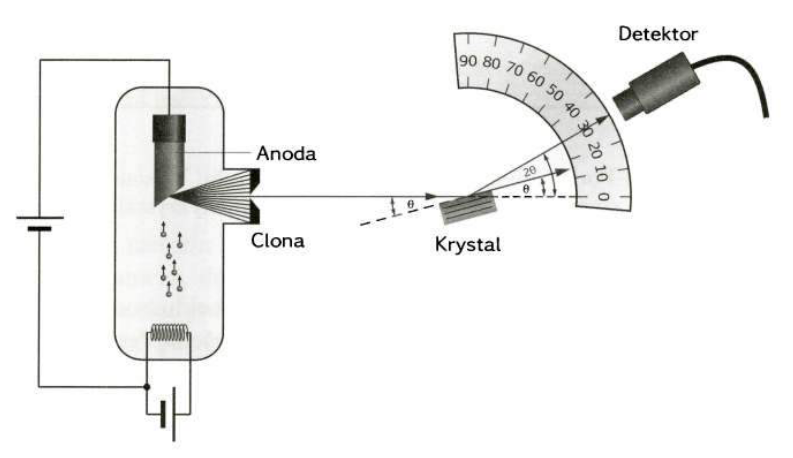
\includegraphics[width=6cm]{danis-bragg.png}
    \caption{Konfigurace Braggovy-Brentanovy metody, převzato z [2].}
    \label{obr:danis-bragg}
\end{wrapfigure}

Naším cílem bude proměřit difrakční obrazec polykrystalického vzorku pomocí Braggovy-Brentanovy metody. Podle difrakčního obrazce budeme následně chtít identifikovat, o jakou látku se jedná.

Při měření Braggovou-Brentanovou metodou měníme úhel $\vartheta$, pod kterým dopadá rentgenové záření na vzorek, a na druhé straně, symetricky také pod úhlem $\vartheta$, detekujeme intenzitu difraktovaného záření. Ve výsledcích z měření se místo úhlu $\vartheta$ často uvádí úhel mezi emitorem a detektorem, který je roven $2\vartheta$. Schéma Braggovy-Brentanovy metody je na obrázku \ref{obr:danis-bragg}.

Při symetrické difrakci na dokonalém krystalu bychom naměřili nenulovou intenzitu $I$ pouze v takových úhlech $\vartheta$, které pro nějaká $h,k,\ell \in \mathbb{N} \cup \{0\}$ splňují tzv. Braggovu difrakční podmínku:
\begin{equation}
    2 \, d_{hk\ell} \, \sin \vartheta = \lambda \: ,
    \label{eq:braggova-podminka}
\end{equation}
kde $\lambda$ je vlnová délka vstupujícího rentgenového záření, $\vartheta$ úhel mezi rovinou vzorku a $d_{hk\ell}$ je mezirovinná vzdálenost roviny s difrakčními indexy $h, k, \ell$. Ve skutečnosti nenaměříme takto ostré hodnoty $I(\vartheta)$ kvůli nedokonalé směrovosti zdroje, nedokonalému úhlovému rozlišení detektoru, konečné velikosti krystalů v práškovém vzorku a přítomnosti nečistot v krystalu. Předpokládáme, že budou teoretické \textit{$\delta$ funkce} konvolučně zhlazené (\textit{gaussovsky} i \textit{lorentzovsky}), a proto očekáváme píky ve tvaru Voigtovy funkce s maximem v hodnotách předpovídaných Braggovou podmínkou.

Budeme měřit krystaly s kubickou mříží, pro které platí vztah:
\begin{equation}
    d_{hk\ell}
    = \frac{2\pi}{\big\lVert \vec{B}_{hk\ell} \big\rVert}
    = \frac{a}{ \! \sqrt{h^2 + k^2 + \ell^2 \,} \, }
    = \frac{a}{J} \: ,
    \label{eq:mezirovinna-vzdalenost}
\end{equation}
kde $a$ je mřížková konstanta a $J \coloneqq \sqrt{h^2 + k^2 + \ell^2 \,}$ je index charakterizující skupinu krystalových rovin se stejnou mezirovinnou vzdáleností. Roviny se stejným $J$ mohou být ekvivalentní a lišit se pouze prostorovou orientací: $$(1,0,0), \; (0,1,0), \; (0,0,1) \: .$$ Také ovšem může jít o neekvivalentní roviny, jejichž mezirovinné vzdálenosti koincidují: $$(3,0,0), \; (2,1,0) \: .$$

V případě primitivní krychlové mříže jsou povoleny všechny hodnoty $h,k,\ell \in \mathbb{N} \cup \{0\}$ a bude tedy možné naměřit píky odpovídající všem kombinacím. U ostatních krychlových mřížích ovšem dochází k tomu, že některé kombinace destruktivně interferují, proto jsou „povolené“ pouze některé kombinace $h,k,\ell$. Přehled povolených kombinací je v tabulce~\ref{tab:kubicke-mrize}.

\phantom{.}
\begin{minipage}{\linewidth}
    \vspace{\baselineskip}
    \centering
    \begin{tabular}{ l|l|l }
        \bfseries typ mříže &
        \bfseries podmínka na $h,k,\ell$ &
        \bfseries hodnoty $J^2$
        \\\hline
        primitivní & libovolná & $1,2,3,4,5, ...$ \\
        prostorově centrovaná & $h+k+\ell = 2n$ & $2,4,6,8,12,...$ \\
        plošně centrovaná & všechna sudá, nebo všechna lichá & $3,4,8,11,12,...$ \\
        typ diamantu & všechna sudá a $h+k+\ell = 4n$, nebo všechna lichá & $3, 11, 16, 19, 20, ...$
    \end{tabular}
    \vspace{0.3\baselineskip}
    \tabcaption{Typy kubických mříží podle [1]}
    \label{tab:kubicke-mrize}
    \vspace{\baselineskip}
\end{minipage}

\noindent
V experimentu naměříme $I(\vartheta)$, identifikujeme píky a pomocí \eqref{eq:braggova-podminka} jim přiřadíme odpovídající hodnoty mezirovinné vzdálenosti $d$. Z těchto hodnot budeme chtít identifikovat, o jaký typ kubické mříže se jedná. K tomu se nám bude hodit hodnota
\begin{equation}
    Q_i
    \coloneqq \frac{ {d_1}^2 }{ {d_i}^2 }
    \approx \frac{ {J_i}^2 }{ {J_1}^2 }
\end{equation}
kde $d_i$ je $i$-tá naměřená hodnota $d$ a $J_i$ je hodnota $J$ příslušící $i$-tému teoreticky naměřitelnému píku. V tabulce \ref{tab:hodnoty-Q} jsou vypsané teoretické hodnoty $Q_i$ pro různé typy mříží.

\phantom{.}
\begin{minipage}{\linewidth}
    \vspace{\baselineskip}
    \centering
    \begin{tabular}{ l|rrrrrrrr }
        \bfseries typ mříže &
        \multicolumn{8}{c}{$Q_i$}
        \\\hline

        primitivní & 1.00 &	2.00 &	3.00 &	4.00 &	5.00 &	6.00 &	8.00 & 9.00 \\
        prostorově centrovaná & 1.00 &	2.00 &	3.00 &	4.00 &	5.00 &	6.00 &	7.00 &	8.00 \\
        plošně centrovaná & 1.00 &	1.33 &	2.66 &	3.67 &	4.00 &	5.33 &	6.33 &	6.67 \\
        typ diamantu & 1.00 &	2.66 &	3.67 &	5.33 &	6.33 &	8.00 &	9.00 &	10.67

    \end{tabular}
    \vspace{0.3\baselineskip}
    \tabcaption{Teoretické hodnoty $Q_i$ pro kubické mříže podle [1]}
    \label{tab:hodnoty-Q}
    \vspace{\baselineskip}
\end{minipage}

Nakonec budeme chtít určit hodnotu mřížkové konstanty $a$. Zdálo by se, že se znalostí $d$ a $J$ ji můžeme přímo vypočítat pomocí vzorce \eqref{eq:mezirovinna-vzdalenost}, tím ovšem dostaneme pouze odhad $a_{\rm e}$, který je zatížený systematickou chybou. Podle [1] pro kubickou mříž platí vztah:
\begin{equation}
    a = a_{\rm e} + s \, \cos \vartheta \, \cot \vartheta \: ,
    \label{eq:mrizkova-konstanta-systematicka-chyba}
\end{equation}
kde $s$ je (neznámá) konsanta úměrnosti.

\section{Výsledky měření}
Naměřená data (viz obrázek \ref{obr:cely-obrazec}) jsme nahráli do programu \textit{WinPLOTR}, ve kterém jsme nalezli polohu píků. Použité rentgenové záření pocházelo z rentgenky s měděnou anodou, proto dostáváme dvojité píky odpovídající dubletům mědi. Při zpracování jsme použili hodnoty výchozí $\lambda$ přednastavené ve WinPLOTRu:
\begin{align*}
    \lambda_1 &= 1.54059803 \U{Å} \\
    \lambda_2 &= 1.54438996 \U{Å}
\end{align*}
Program WinPLOTR z důvodu numerické náročnosti používal pro fitování pseudo-Voigtovu funkci, která je lineární kombinací Gaussovy a Lorentzovy funkce (místo teoreticky předpovídané Voigtovy funkce, která je jejich \textit{konvolucí}). Volné parametry fitu píků byly: hodnota šumu nalevo a napravo od píku, poloha maxima, FWHM, intenzita píku a parametr $\eta$ pseudo-Voigtovy funkce. Detail jednoho z fitů je na obrázku \ref{obr:fit-peaku}.

\phantom{.}\\[-\baselineskip]
\begin{minipage}{\linewidth}
    \vspace{\baselineskip}
    \centering
    \def\gptboxheight{17cm}
    \begin{gnuplot}[terminal=epslatex,terminaloptions={color size 17cm, 8cm}]
        set xrange [30:110]
        set xlabel '$2 \vartheta \; [\°]$'
        set ylabel '$I$'
        plot 'data-default/dataset021_Cu.dat' using (10 + $0*0.02):($1/100) w l not
    \end{gnuplot}
    \vspace{-\baselineskip}
    \figcaption{Naměřený difrakční obrazec}
    \label{obr:cely-obrazec}
    \vspace{\baselineskip}
\end{minipage}

\phantom{.}\\[-\baselineskip]
\begin{minipage}{\linewidth}
    \vspace{\baselineskip}
    \centering
    \begin{tabular}{ rl|r|rl|rl|rl }
        \multicolumn{2}{c|}{ $2\vartheta \; [\U{\°}]$ } &
        \multicolumn{1}{c|}{ $d \; [\U{Å}]$ } &
        \multicolumn{2}{c|}{ $ I $ } &
        \multicolumn{2}{c|}{ FWHM $[\U{\°}]$ } &
        \multicolumn{2}{c}{ $\eta$ }
        \csvreader[ head to column names ]{peaky-data.csv}{}
        {
            \csviffirstrow{\\\hline}{\\}
            \uhel & $\hspace{-1em} \pm$ \uhelerr &
            \vzdalenost &
            \intenzita & $\hspace{-1em} \pm$ \intenzitaerr &
            \FWHM & $\hspace{-1em} \pm$ \FWHMerr &
            \eta & $\hspace{-1em} \pm$ \etaerr
        }
    \end{tabular}
    \vspace{0.5\baselineskip}
    \tabcaption{Výstup programu WinPLOTR}
    \label{tab:peaks-data}
    \vspace{\baselineskip}
\end{minipage}

\begin{wrapfigure}{r}{7cm}
    \centering
    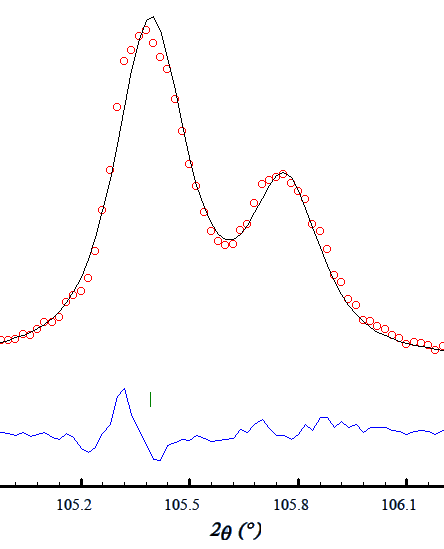
\includegraphics[width=6cm]{peak-fit.png}
    \caption{Detail píku na $2\vartheta = 105\°$. Červené kruhy značí naměřená data, černá spojitá čára fit pseudo-Voigtovou funkcí, fialovomodrá čára pod grafem ukazuje rozdíl fitu a naměřených dat. Vidíme, že naměřený pík je asymetrický – oproti fitu je nakloněný doleva.}
    \label{obr:fit-peaku}
    \vspace{\baselineskip}

    \def\gptboxheight{7cm}
    \begin{gnuplot}[terminal=epslatex,terminaloptions={color size 6cm, 6cm}]
        set datafile separator ','

        a=s=1
        f(x) = -s*x + a
        fit f(x) 'systematicka-chyba-data.csv' skip 1 via a,s

        set key left top
        set xlabel '$\cos\vartheta \, \cot\vartheta$'
        set ylabel '$a_{\rm e} \; [\U{Å}]$' offset 1.5,0,0
        set xrange [-0.2:1.5]
        set yrange [4.32:4.36]
        set xtics 0,0.5
        set ytics 4.32,0.01
        set lmargin 5
        set rmargin 0
        plot 'systematicka-chyba-data.csv' skip 1 t 'data', f(x) t 'fit'
    \end{gnuplot}
    \vspace{-0.3\baselineskip}
    \figcaption{Lineární regrese odhadů mřížkové konstanty v závislosti na předpokládané systematické chybě}
    \label{obr:systematicka-chyba-fit}
    \vspace{-12\baselineskip}
\end{wrapfigure}
\noindent
Výstupní data z programu WinPLOTR jsou v tabulce \ref{tab:peaks-data}, společně s vypočítanou mřížkovou vzdáleností $d$ odpovídající naměřenému $2\vartheta$. Chybu $d$ můžeme dopočítat pomocí vzorce pro propagaci malé chyby z \eqref{eq:braggova-podminka} jako:
\begin{equation*}
    \sigma(d)
    = d \;
    \frac{
        \, \sigma(\vartheta) \,
    }{
        \vartheta
    }
\end{equation*}
Dále jsme podle \eqref{tab:hodnoty-Q} dopočítali hodnoty $Q_i$. Vyšlo nám:

\phantom{.}\\[-\baselineskip]
\begin{minipage}{10cm}
    \vspace{\baselineskip}
    \centering
    \begin{tabular}{cccccccc}
        1.00 &
        1.34 &
        2.68 &
        3.69 &
        4.02 &
        5.37 &
        6.37 &
        6.71
    \end{tabular}
    \vspace{\baselineskip}
\end{minipage}

\noindent
Porovnáním s tabulkou \ref{tab:hodnoty-Q} jsme zjistili, že naměřená data velmi dobře odpovídají plošně centrované kubické mříži.

Protože z tabulky \ref{tab:kubicke-mrize} víme, že první naměřitelný pík plošně centrované mřížky má index ${J_1 = 3}$, můžeme snadno dopočítat $J_i$ pro všechny naměřené hodnoty $d_i$:
\begin{equation*}
    J_i \approx \sqrt{3 \, Q_i}
\end{equation*}
Teď už můžeme podle vzorce \eqref{eq:mezirovinna-vzdalenost} vypočítat $a_{\rm e}$. Dostáváme hodnoty:

\phantom{.}\\[-\baselineskip]
\begin{minipage}{10cm}
    \vspace{\baselineskip}
    \centering
    \begin{tabular}{rl|r|rl}
        \multicolumn{2}{c|}{$d \; [\U{Å}]$} &
        \multicolumn{1}{c|}{$J$} &
        \multicolumn{2}{c}{$a_{\rm e} \; [\U{Å}]$}
        \csvreader[ head to column names ]{mrizkova-konstanta-data.csv}{}{
            \csviffirstrow{\\\hline}{\\}
            \mezirov & $\hspace{-1em} \pm$ \meziroverr &
            \index &
            \mrizk & $\hspace{-1em} \pm$ \mrizkerr
        }
    \end{tabular}
    \vspace{0.5\baselineskip}
    \tabcaption{Vypočítané odhady mřížkové konstanty}
    \label{tab:mrizkova-konstanta-odhady}
    \vspace{\baselineskip}
\end{minipage}

\noindent
Úpravou vztahu \eqref{eq:mrizkova-konstanta-systematicka-chyba} získáme závislost vhodnout pro lineární regresi:
\begin{equation*}
    a_{\rm e} = -s \, \cos\vartheta \, \cot\vartheta + a
\end{equation*}
Odhady $a_{\rm e}$ v závislosti na $\cos\vartheta \, \cot\vartheta$ jsme vynesli do grafu v obrázku \ref{obr:systematicka-chyba-fit} a proložili přímkou. Tím jsme dostali hodnoty:
\begin{align*}
    a &= (4.3312 \pm 0.0006) \U{Å} \\
    s &= \hspace{2pt} (-0.012 \pm 0.001) \U{Å}
\end{align*}
Nakonec seřadíme naměřené píky podle intenzity a provnáme je s krystalografickými tabulkami pro látky s plošně cetrovanou kubickou mříží – to je poměrně účinný způsob, jak určit, jakou látkou je náš vzorek tvořen. Toto porovnání pro nejpodobnější látky je v tabulce \ref{tab:porovnani-intenzit}.

\pagebreak

\phantom{.}\\[-\baselineskip]
\begin{minipage}{\linewidth}
    \vspace{\baselineskip}
    \centering
    \begin{tabular}{cc|ccc}
        $I$ & $d \; [\U{Å}]$ &
        MnO & TiC & FeO
        \csvreader[ head to column names ]{intenzita.csv}{}{
            \csviffirstrow{\\\hline}{\\}
            \inten &
            \mrizk &
            \MnO & \TiC & \FeO
        }
    \end{tabular}
    \vspace{\baselineskip}
    \tabcaption{Porovnání difrakčních maxim s krystalografickými tabulkami [3]}
    \label{tab:porovnani-intenzit}
    \vspace{\baselineskip}
\end{minipage}

\noindent
Až na poslední hodnotu naměřená data velmi dobře odpovídají TiO. Podle tabulek [3] má TiO plošně centrovanou mříž s mřížkovou konstantou:
\begin{equation*}
    a = 4.3274 \U{Å}
\end{equation*}


\section{Diskuse}
Jak je vidět v obrázku \ref{obr:fit-peaku}, konvoluční zhlazení ostrých hodnot, které předpovídá Braggova podmínka, nebylo \textit{voigtovské}, jak jsme předpokládali v teorii, ale asymetrické. To do všech vypočítaných hodnot ($\vartheta, d, a_{\rm e}, a$) zaneslo systematickou chybu, kterou jsme nedokázali odstranit. Důvod takového asymetrického zhlazení není autorovi zřejmý, mimo jiné proto, že mu nejsou známy okolnosti měření tohoto vzorku.



\section{Závěr}
Z naměřených dat se podařilo odečíst hodnoty difrakčních maxim. Z nich se podařilo vypočítat mezirovinné vzdálenosti $d$, určit, že vzorek má plošně centrovanou mřížkum, a následně vypočítat odhady mřížkové konstanty $a_{\rm e}$ pro jednotlivé píky.
Podařilo se kvantifikovat systematickou chybu způsobenou instrumentálními efekty jako:
\begin{equation*}
    a = a_{\rm e} + (-0.012 \pm 0.001) \U{Å} \; \cdot \; \cos \vartheta \, \cot \vartheta \: .
\end{equation*}
Po započítání této systematické chyby jsme určili nejlepší odhad mřížkové konstanty:
\begin{equation*}
    a = (4.3312 \pm 0.0006) \U{Å} \: .
\end{equation*}
Pomocí krystalografických tabulek se podařilo určit, že vzorek byl TiC, jehož tabulková mřížková konstanta je:
\begin{equation*}
    a = 4.3274 \U{Å} \: .
\end{equation*}
Námi určená hodnota není v souladu s tabulkovou hodnotou, konkrétně je naměřená hodnota o 0.8~\textperthousand $\;$ vyšší než tabulková hodnota, ačkoliv její statistická chyba je pouze 0.1~\textperthousand.

\section{Literatura}
[1] Praktikum částicové a jaderné fyziky. Objevování částic v detektoru ATLAS v CERN. \\ Dostupné z: \url{https://physics.mff.cuni.cz/vyuka/zfp/_media/zadani/texty/txt_401.pdf}. 26. září 2019.
\\\\
{}[2] DANIŠ, Stanislav. \textit{Atomová fyzika a elektronová struktura látek.} Praha: MatfyzPress, 2019. \\ ISBN 978-80-7378-376-1. Kapitola Struktura pevných látek.
\\\\
{}[3] SWANSON, H.E. and E. Tatge. \textit{Standard X-ray Difraction Powder Patterns.} National Bureau of Standards. 1953.

\end{document}
